\section{Final remarks and outlook}

The use the ALICE detector material as a target for measuring antinuclei annihilations by means of their inelastic cross sections has proven a fruitful way to conduct these otherwise challenging measurements. Yet the potential of these measurement techniques is far from exhausted. In this section I want to highlight what has already been achieved (not just by me in this thesis, but also by other works), and talk about the progress still to come. \\

\subsection{Measurements of the inelastic cross sections of antinuclei}

The full list of the inelastic cross section measurements using both the antiparticle-to-particle method and the TOF-to-TPC method are shown in figure \ref{fig:AntinucleiInelasticCross_Sections_Full}. For antideuterons, this represents the first low energy measurement of the inelastic cross section, while for \ahe\ and \atrit\ it is the very first measurement of the inelastic cross sections ever. In the upcoming Run 3 and Run 4 data taking campaigns at the LHC, we will be able to drastically reduce the statistical uncertainties dominating for the $A$ = 3 antinuclei, and hopefully extend this set of measurements to $A$ = 4 antinuclei. Indeed, in Run 3 the expected increase in statistics for Pb--Pb collisions is a factor 100. Considering the penalty factor per additional nucleon in Pb--Pb collisions, this would result in statistical uncertainties for the measurement of the inelastic cross sections of $A$ = 4 antinuclei only $\sqrt{3.5}$ times larger than the uncertainties on the $A$ = 3 results already measured, making such measurements highly feasible. Additionally, by updating studies on the material budget and improving our secondary distributions in Monte Carlo, the statistical uncertainties are expected to be significantly reduced, so that hopefully we will be able to make precision measurements of these cross sections. Furthermore, there are plans to include a target material in the ALICE detector, in order to probe the annihilation of particles on different materials directly. With this exciting experimental development -- and the ever improving understanding of the nature of the strong force due to femtoscopy measurements \cite{Three_body_femto} %cite the p-d paper (in prep?) and the 3 body paper, as well as the nature paper. 
we hope to inspire new theoretical work on the topic of antinuclei annihilations, and maybe finally even a theoretical framework to describe its low energy behavior. \\

\begin{figure}
    \centering
    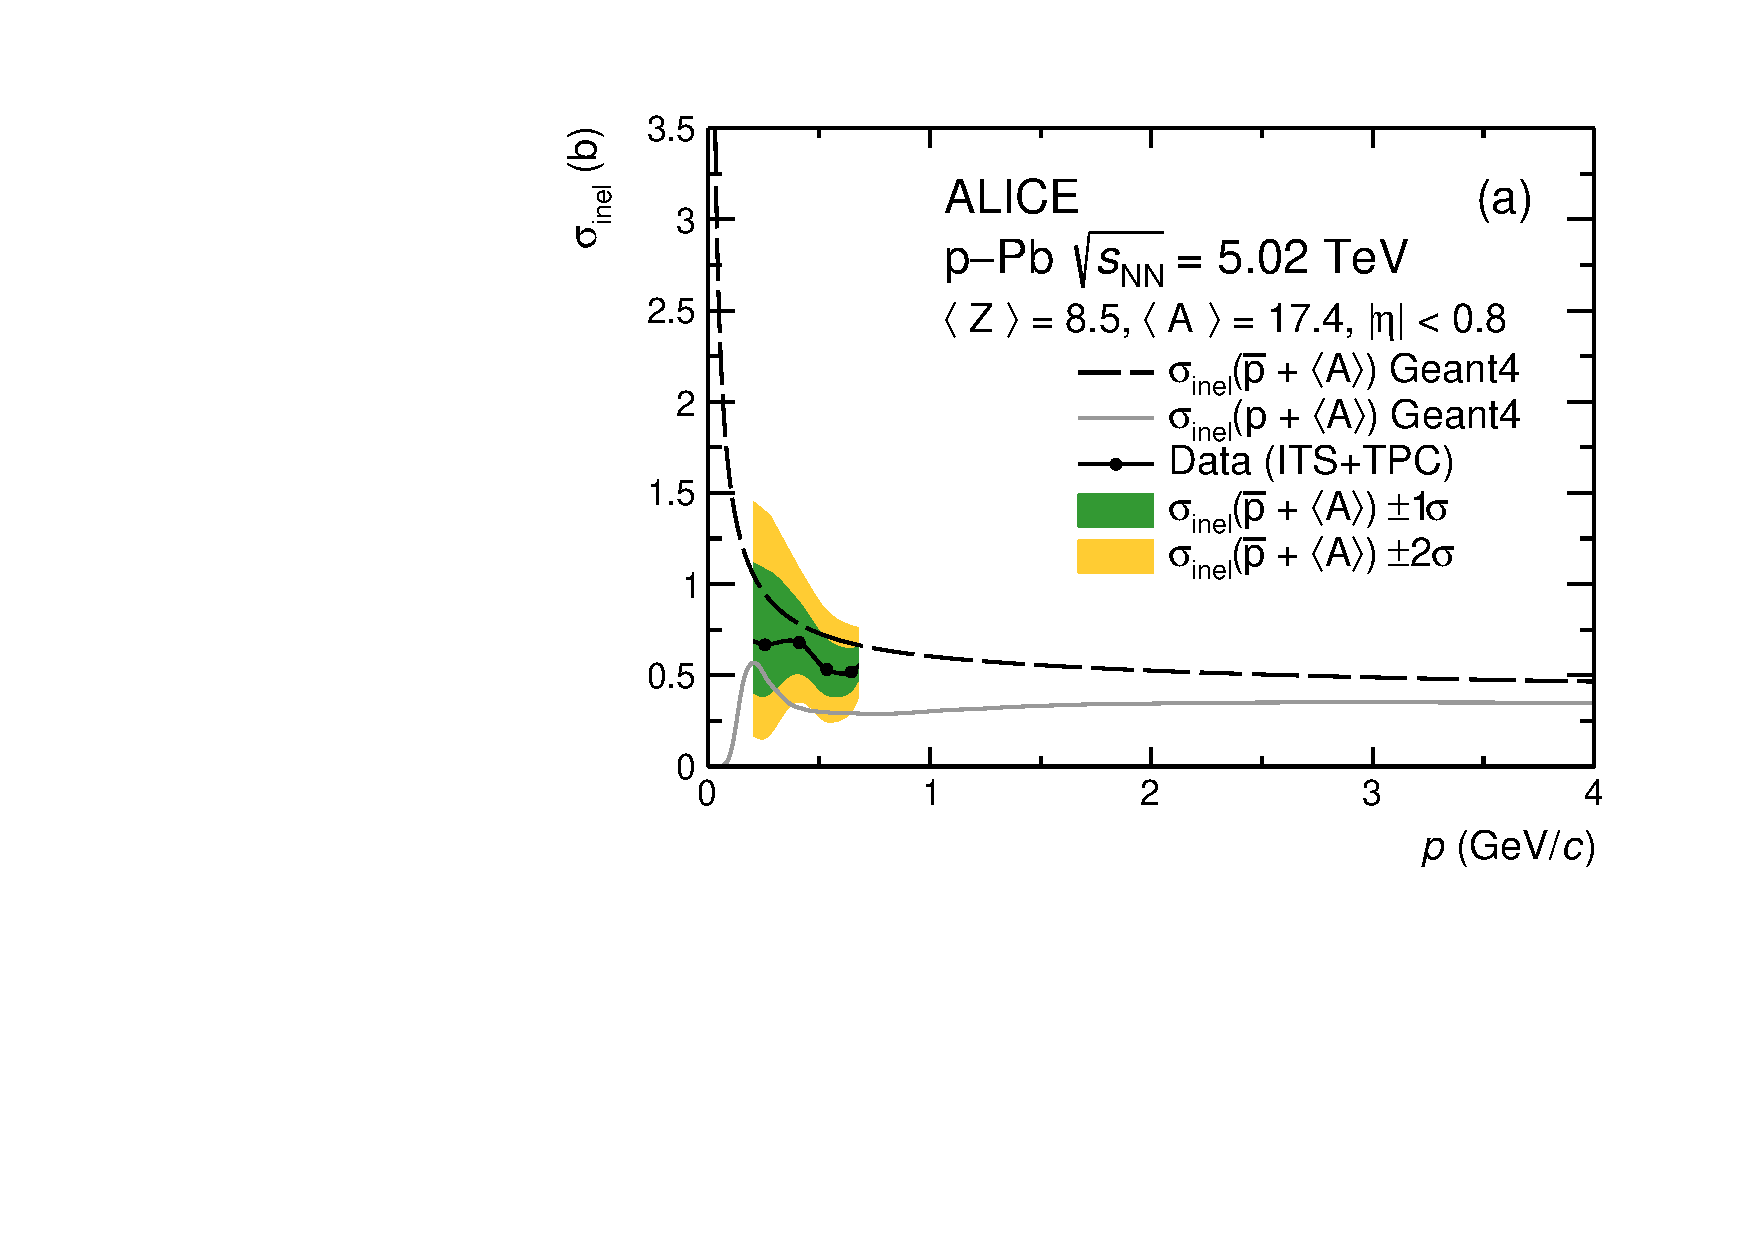
\includegraphics[width=0.48\textwidth]{figures/CS_antip_ALICE_ITSTPC.pdf}
    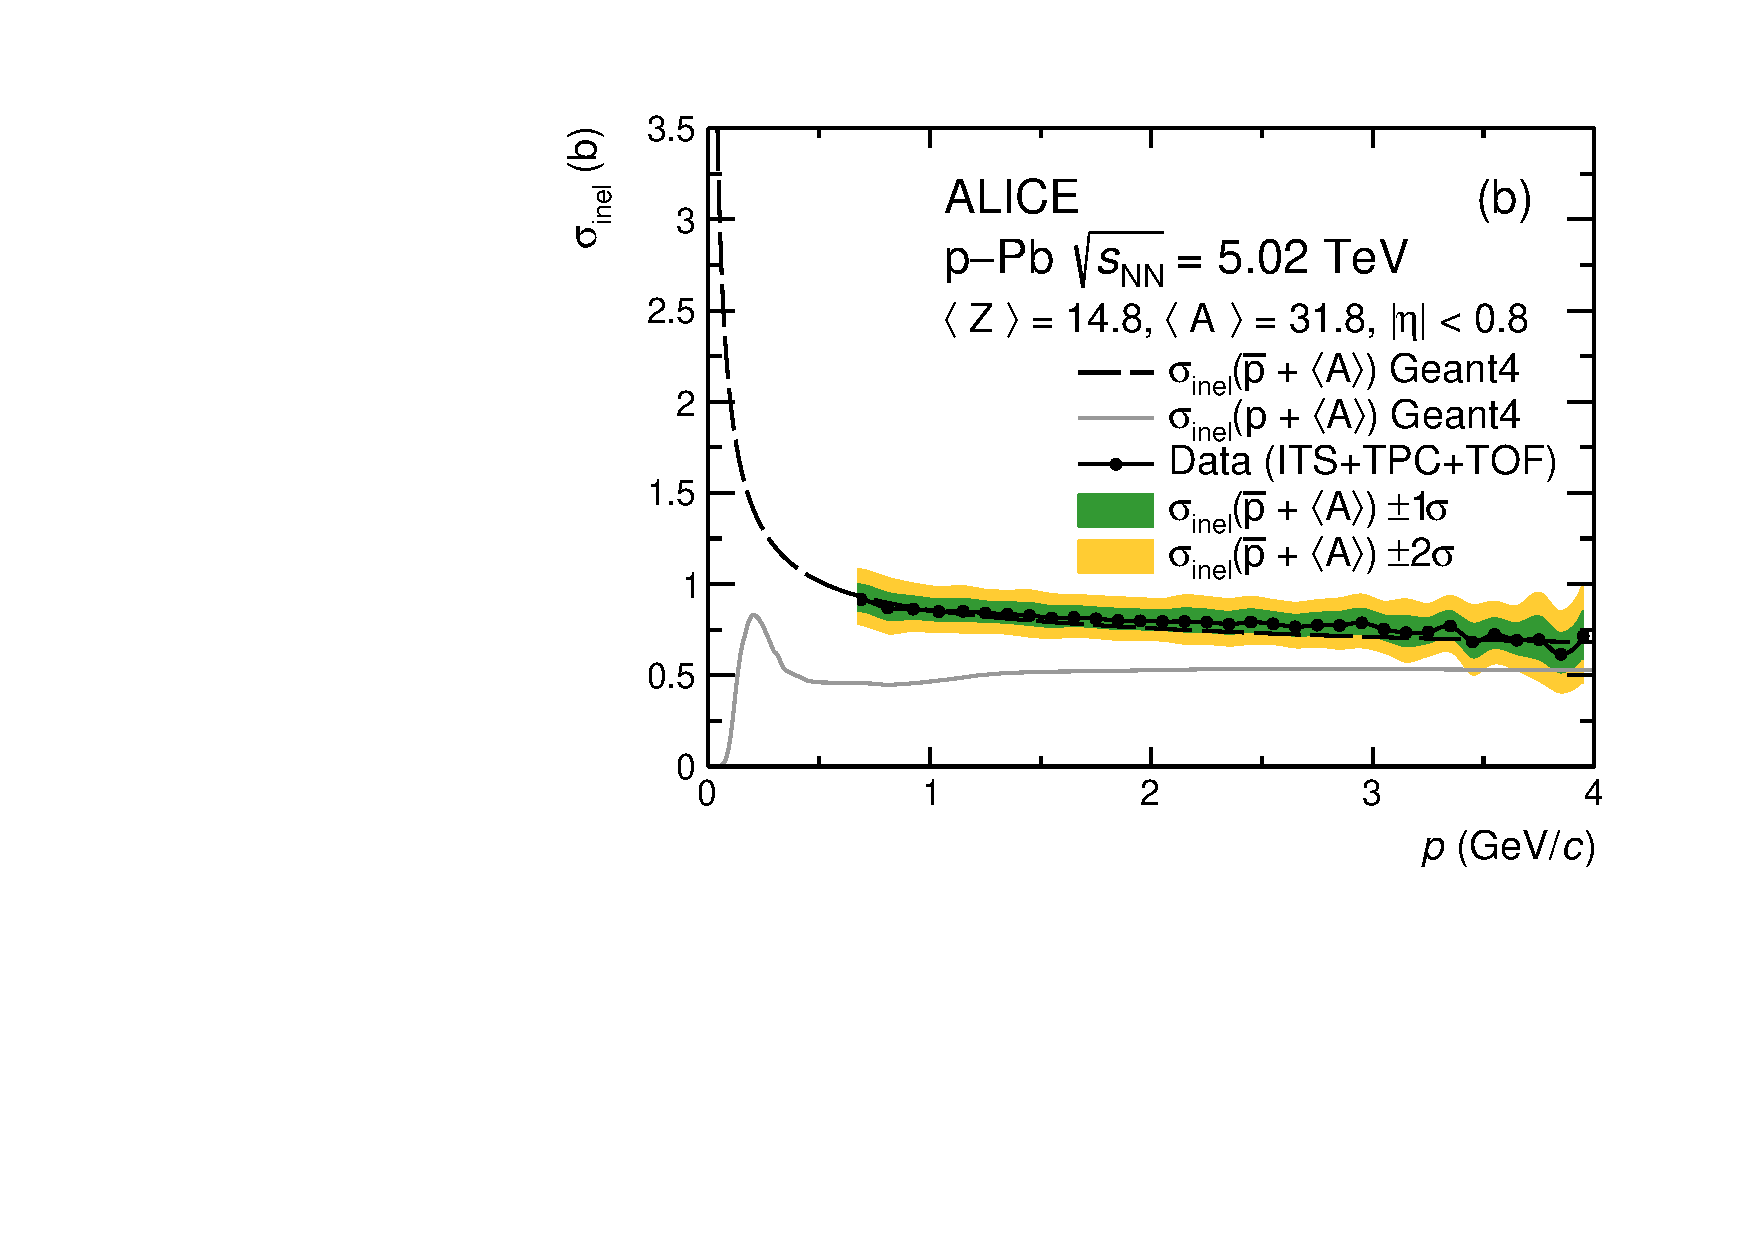
\includegraphics[width=0.48\textwidth]{figures/CS_antip_ALICE_TOF.pdf}
    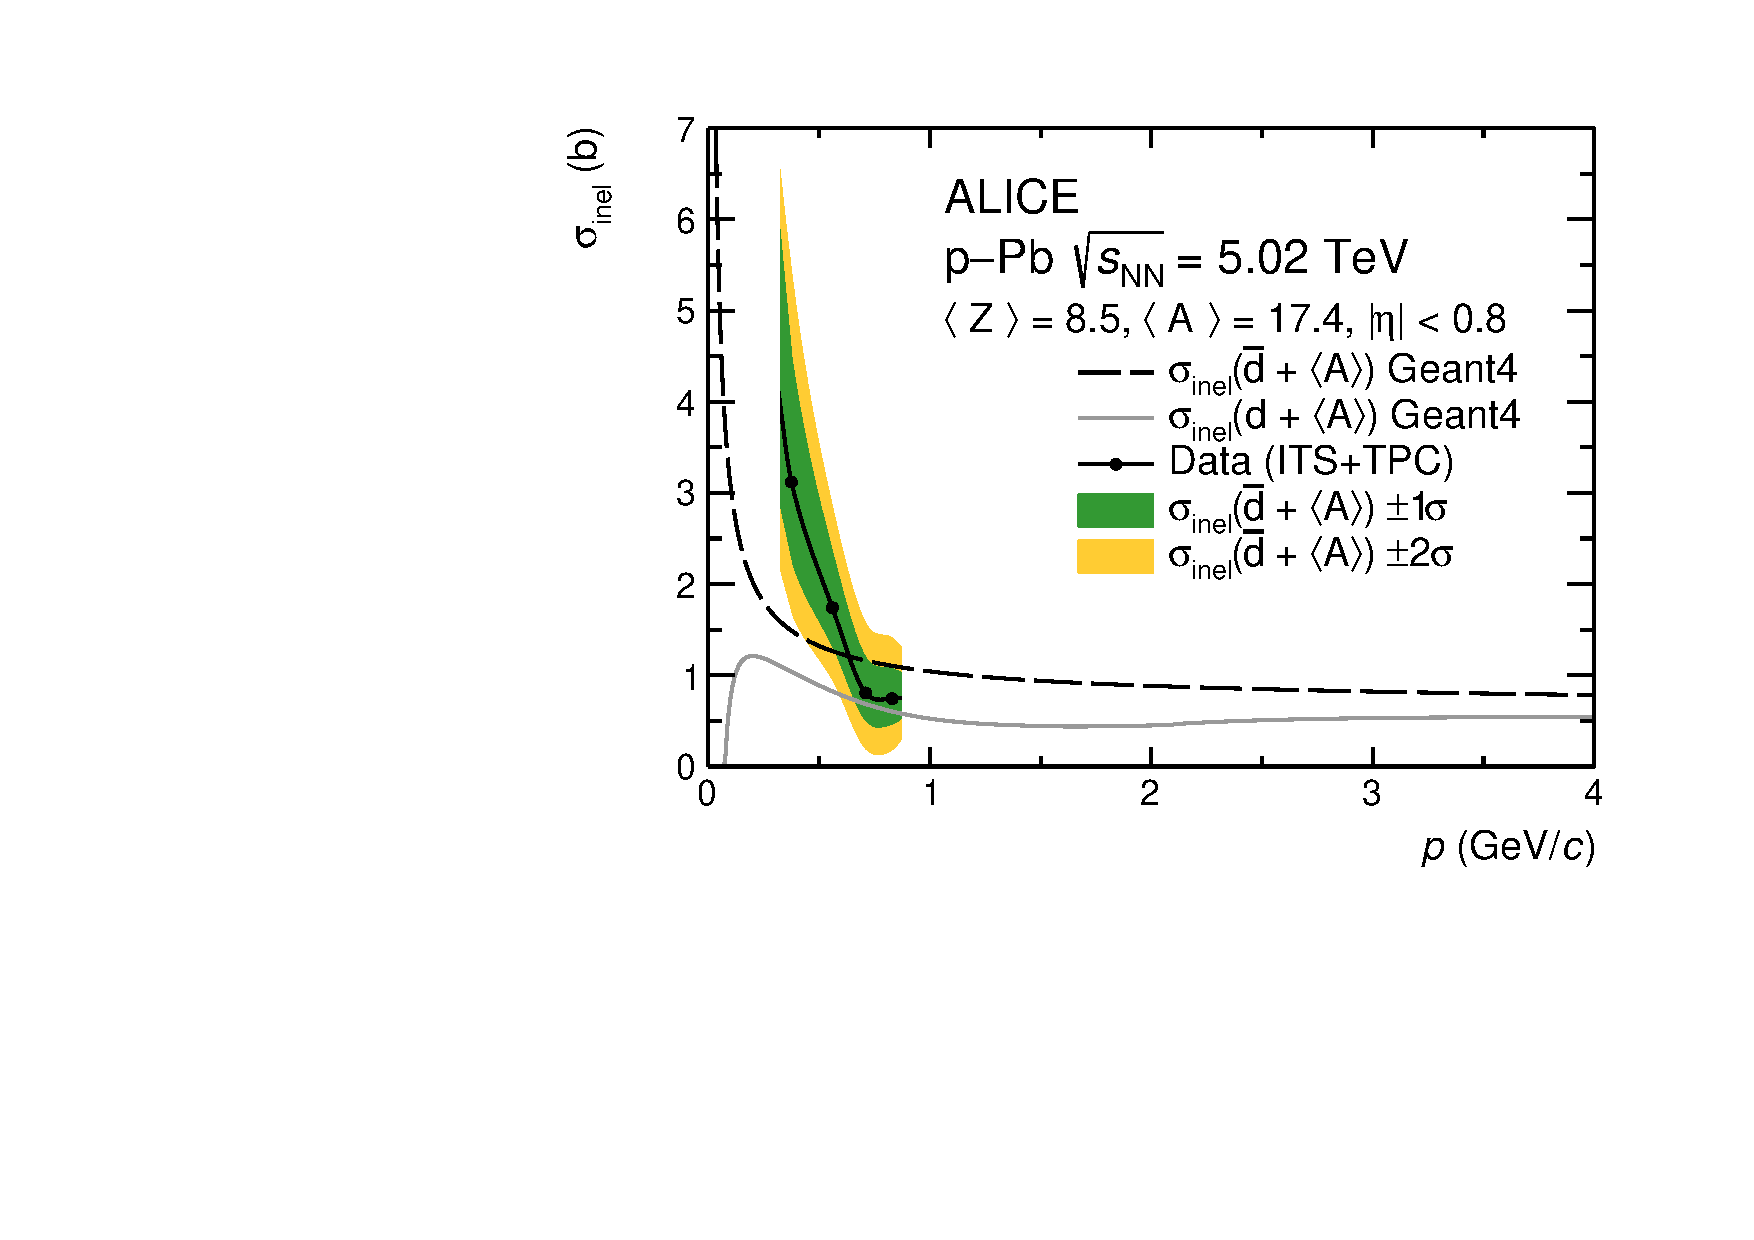
\includegraphics[width=0.48\textwidth]{figures/CS_antid_ALICE_fullMC_ITSTPC_noc.pdf}
    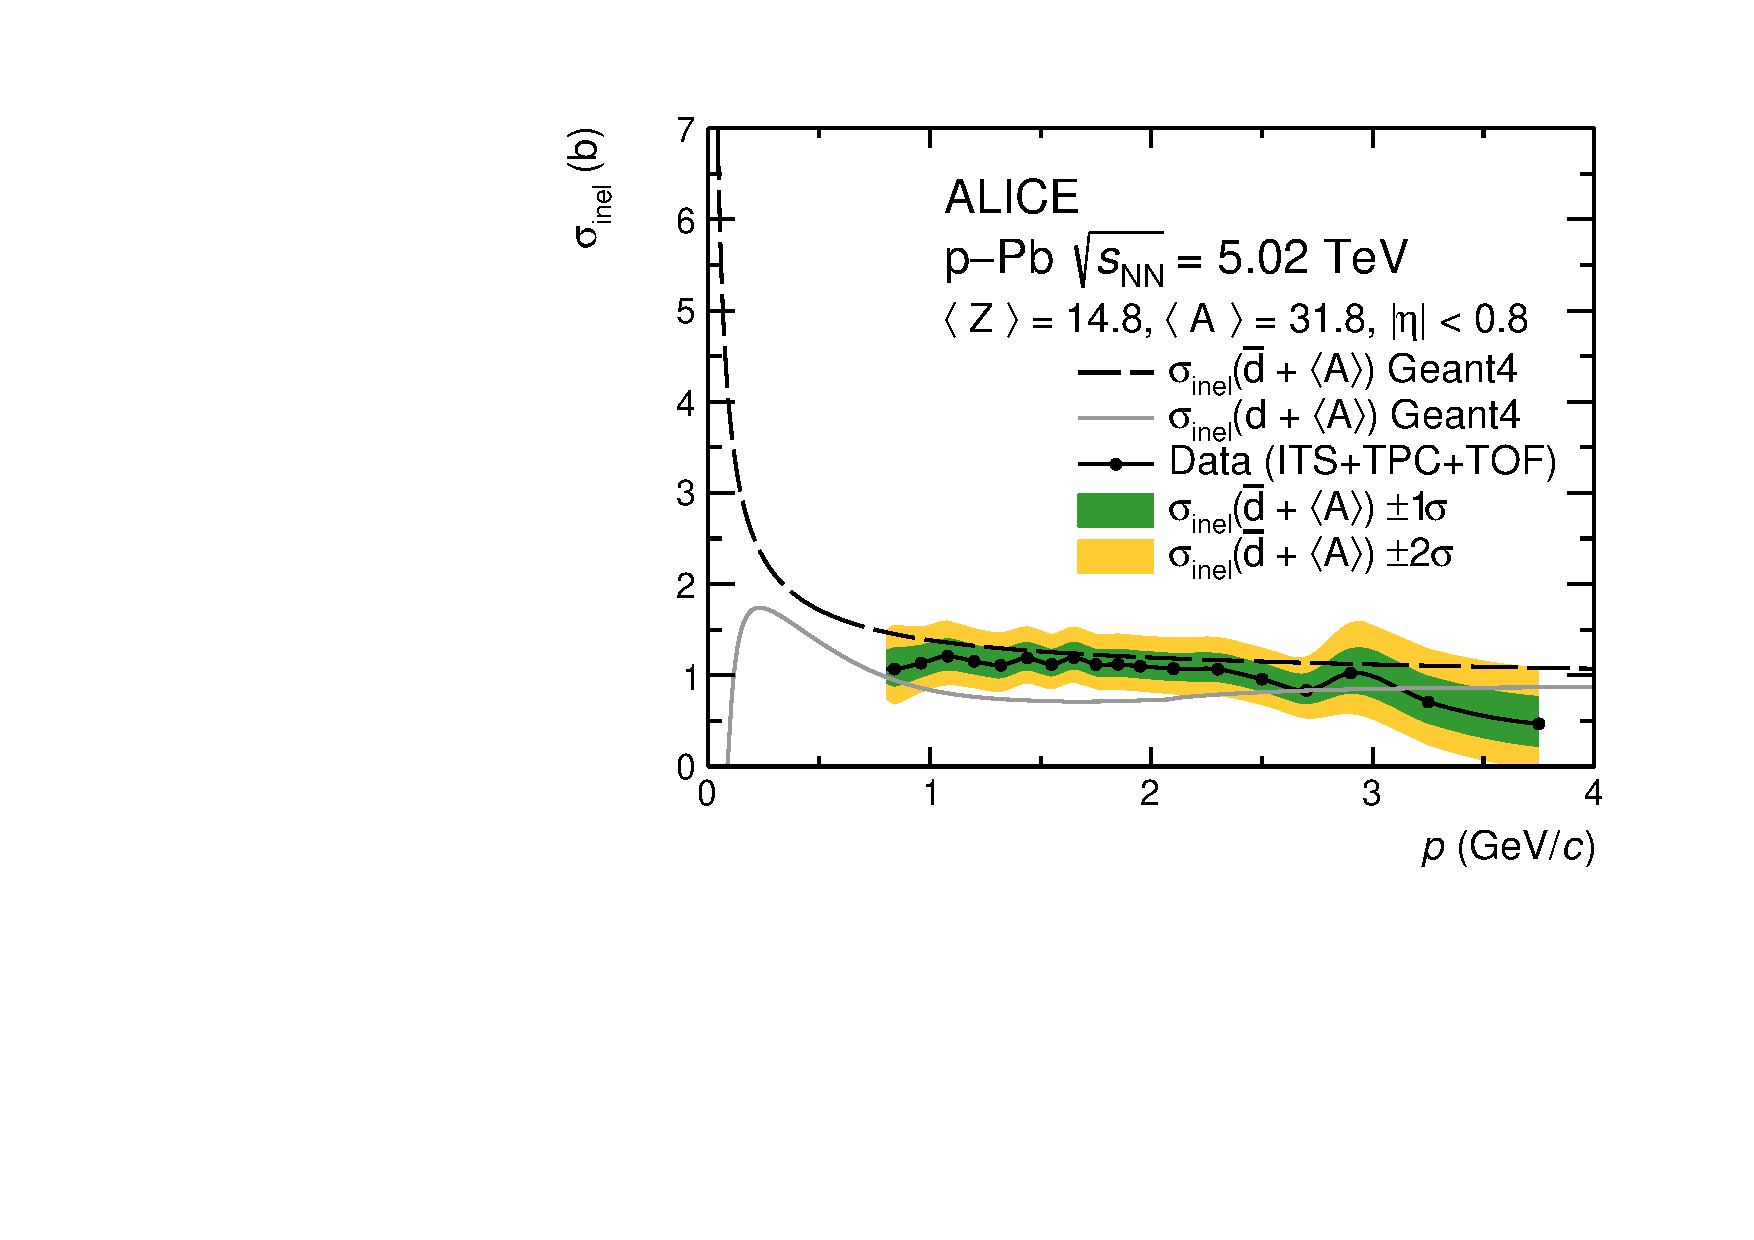
\includegraphics[width=0.48\textwidth]{figures/CS_antid_ALICE_fullMC_TOF_nod.pdf}
    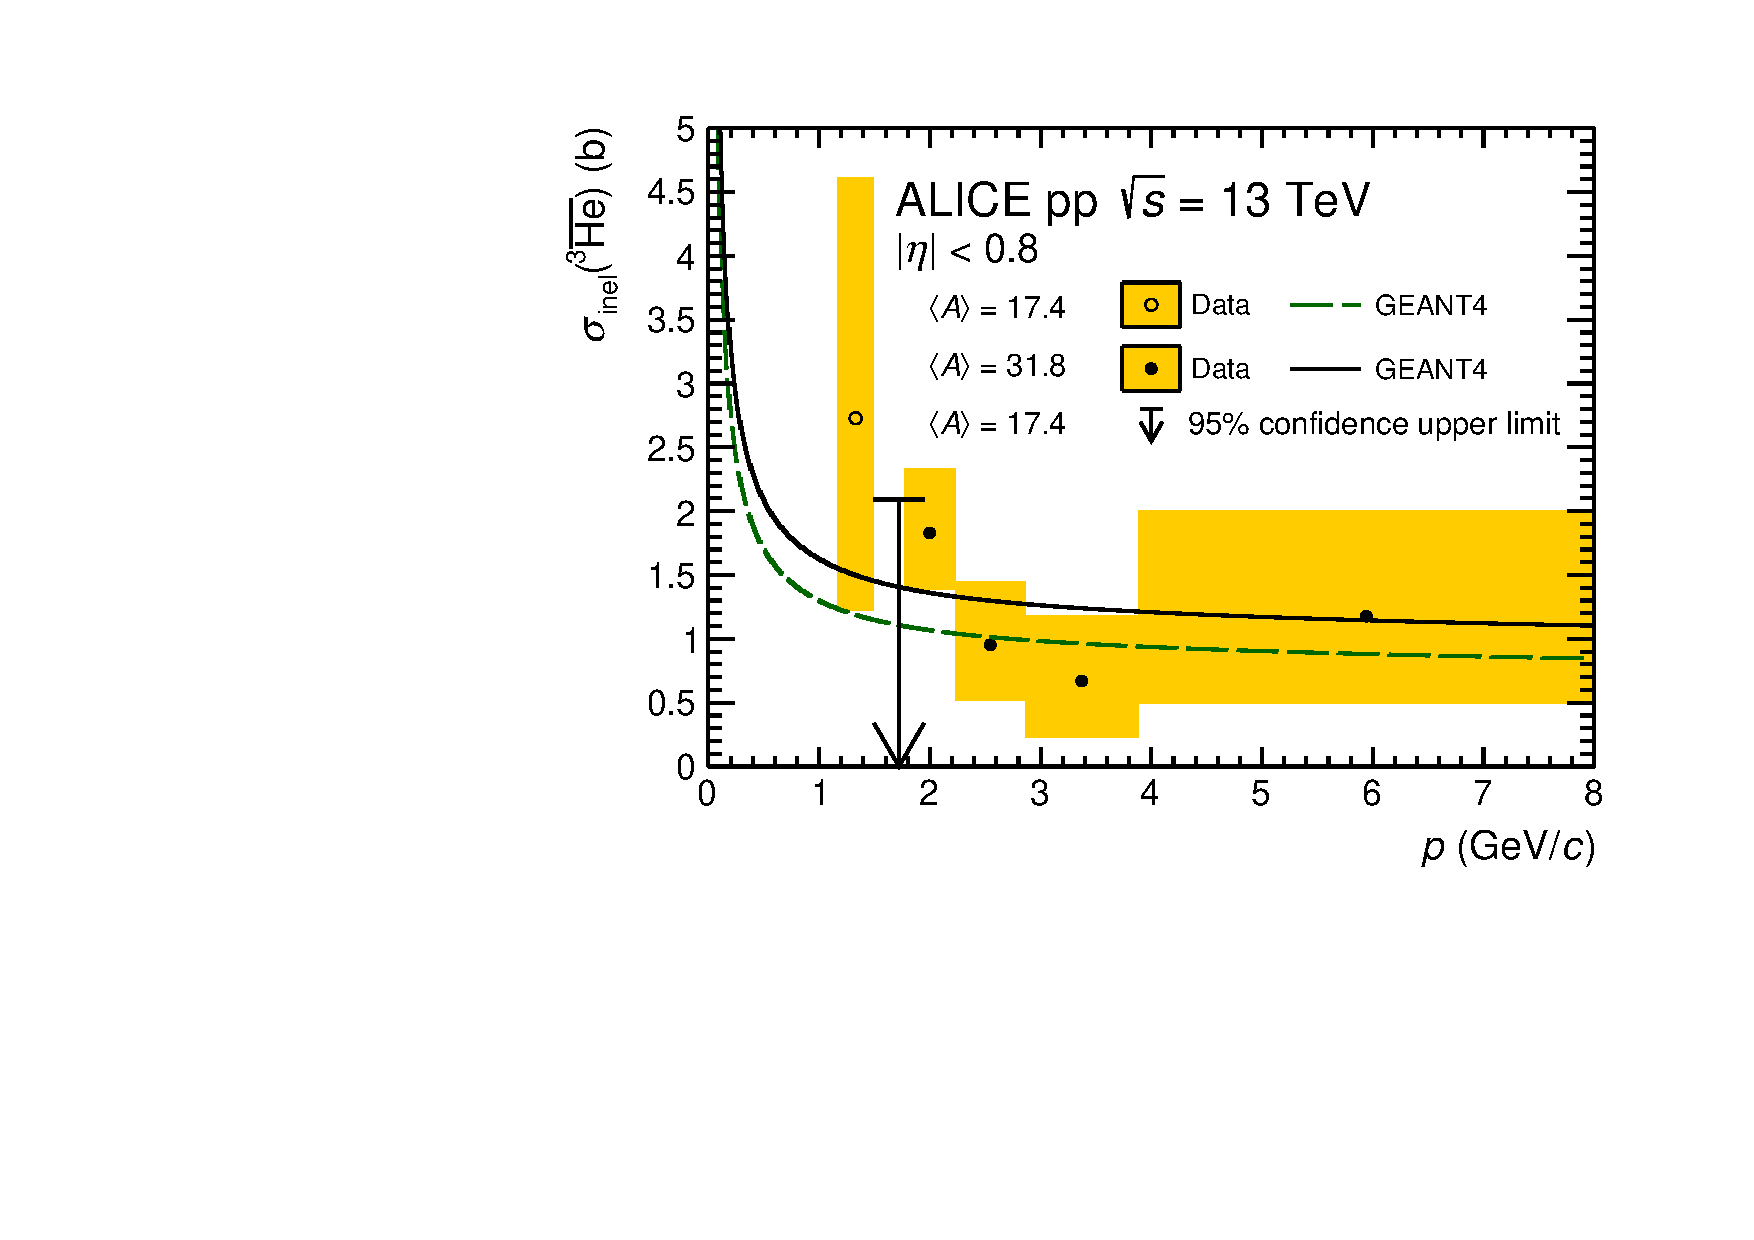
\includegraphics[width=0.48\textwidth]{figures/Antihelium_inelastic_cross_section.pdf}
    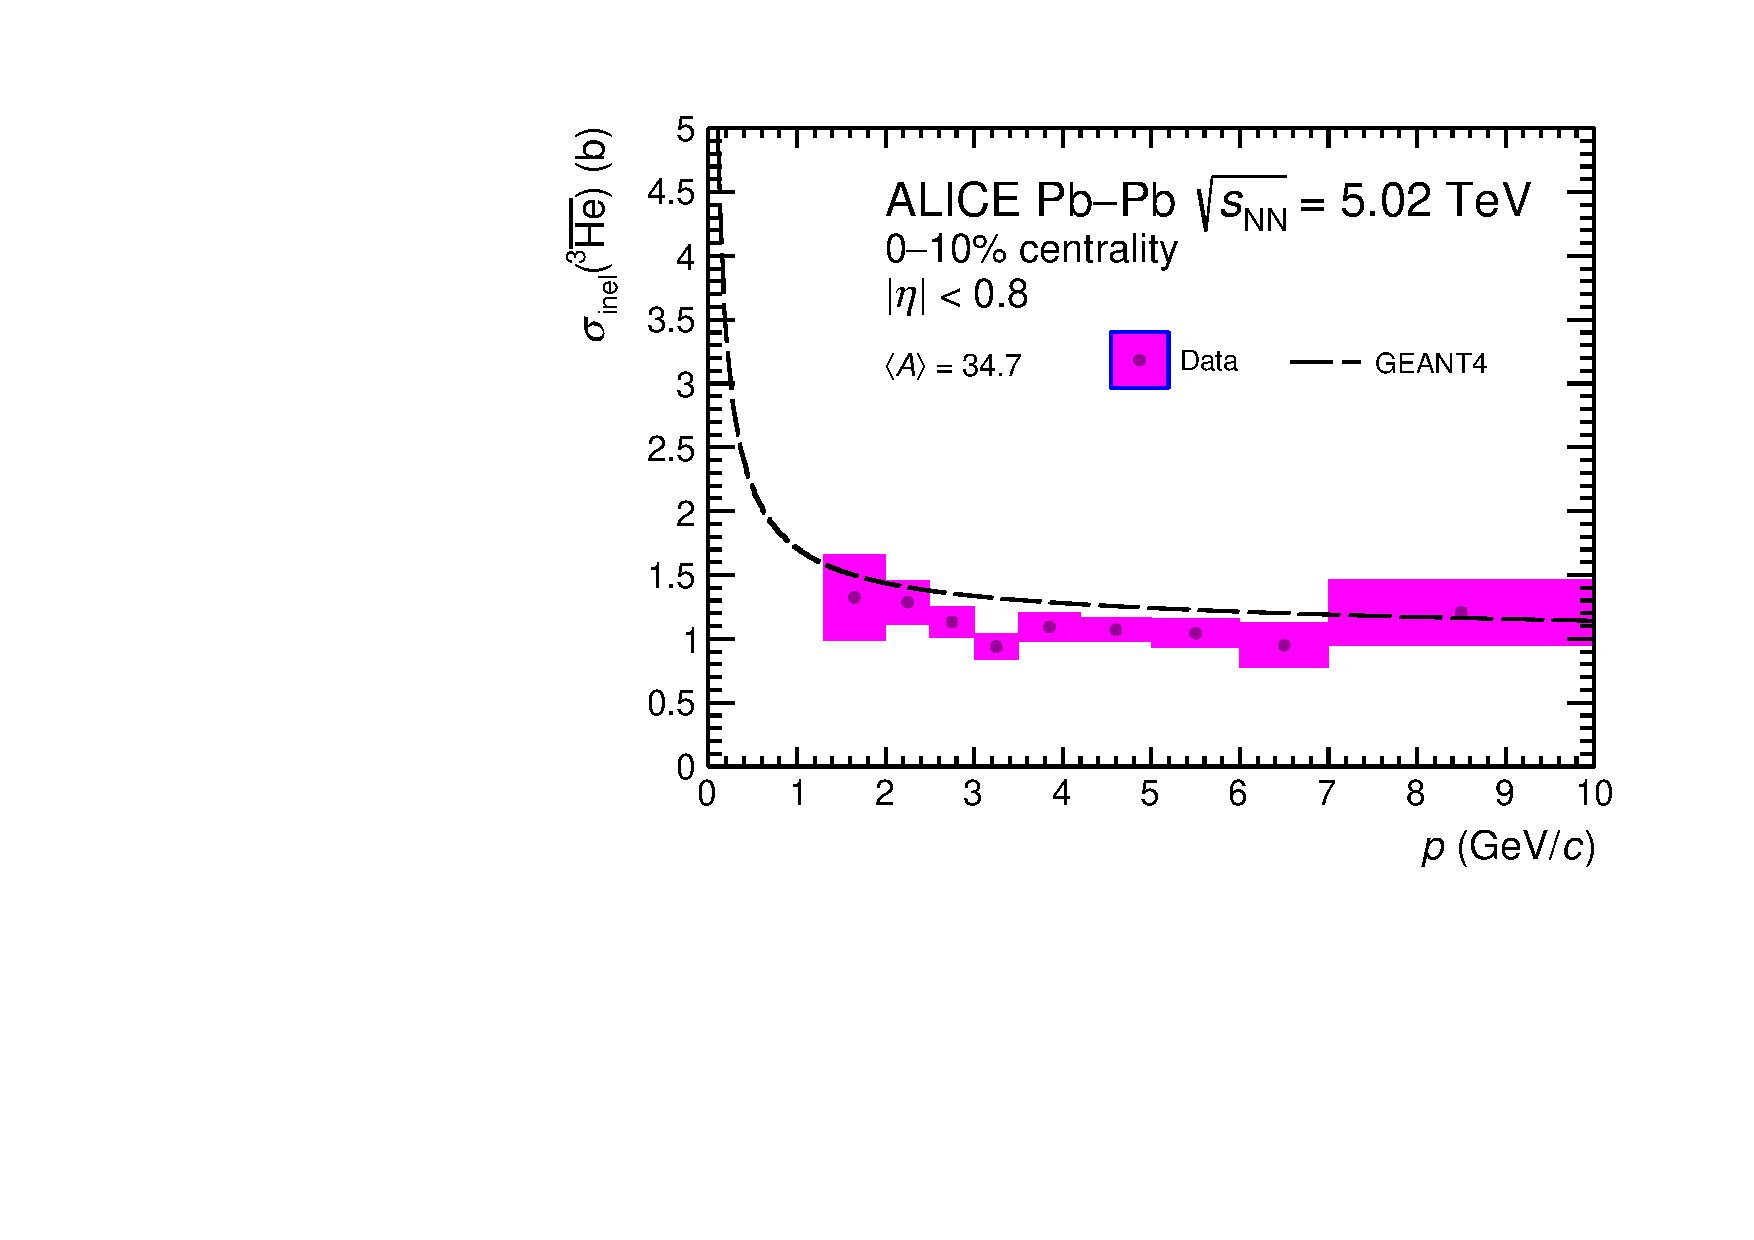
\includegraphics[width=0.48\textwidth]{figures/Antihelium_inelastic_cross_section_PbPb.pdf}
    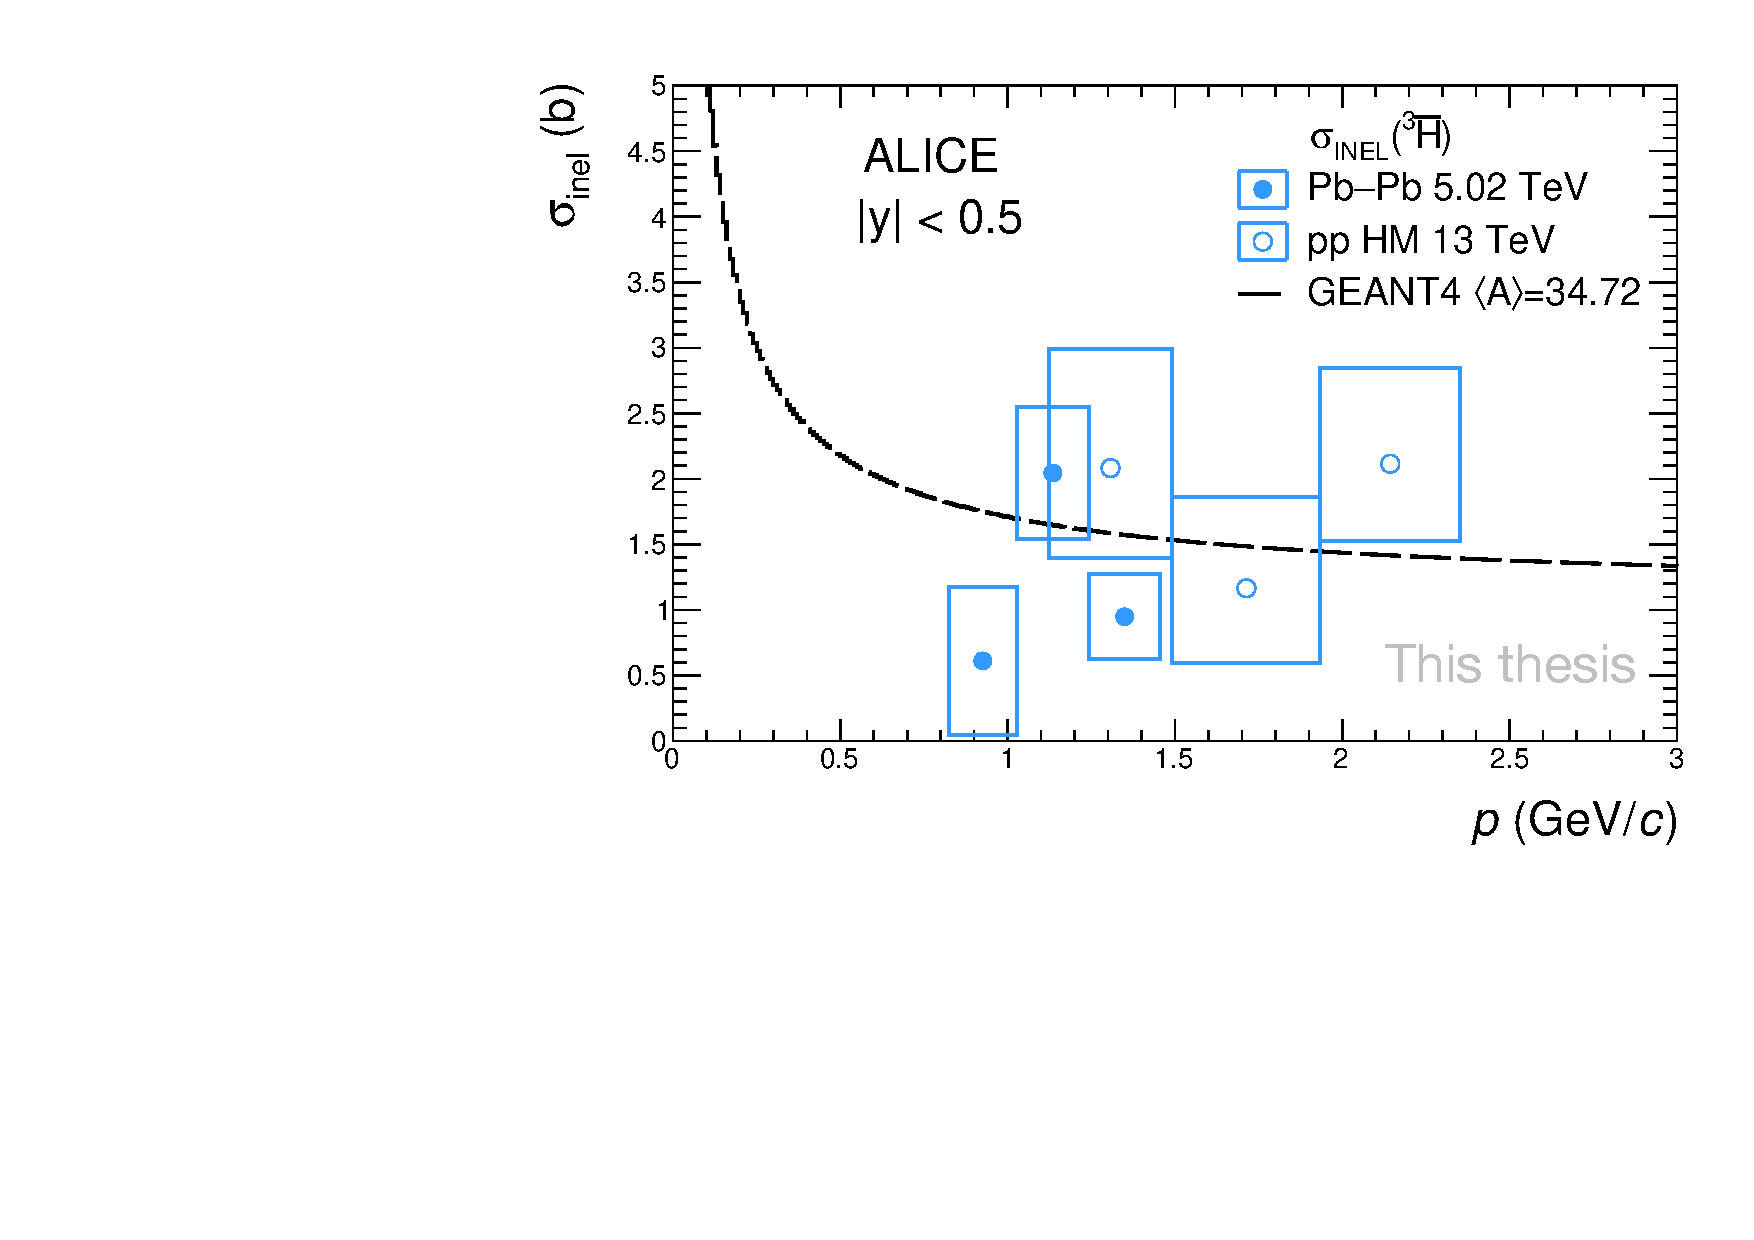
\includegraphics[width=0.48\textwidth]{figures/FinalXS_antit_paper.pdf}
    \caption{The inelastic cross section measurements for the antinuclei from $A$ = 1 to $A$ = 3, as measured by ALICE in \cite{antideuteronXS, antiHe3XS} and in an upcoming publication on \atrit\ . }
    \label{fig:AntinucleiInelasticCross_Sections_Full}
\end{figure}

\subsection{Use of these measurements}
In nuclear physics, the principal use of these cross sections is twofold. The first use is a more accurate description of antinuclei propagation using Geant4, once the Geant4 parameterizations are adjusted with these new results. Additionally, these measurements allow the assignment of an experimental uncertainty due to these measurements. Ideally, this would allow the study of antinuclei production to lower momenta than is currently common practice \cite{4He_production, helium3_flow_5TeV, deuteron_pp_13TeV, deuteron_pp_7TeV, deuteron_PbPb_276TeV, deuteron_pPbALICE}. The second use is a new probe into the isospin dependence of the strong force, using two charged particles in \ahe\ and \atrit\ . With future precision measurements, any possible discrepancy between these isospin partners will complement existing studies using the antiproton and antineutron inelastic cross sections \cite{Bianconi_2014}.\\


But the main use of these measurements is in another field: astrophysical dark matter searches using antinuclei. The work done as part of this thesis has shown the effect of the annihilation on the expected antinuclei fluxes and determined an experimental uncertainty on the transparency of our galaxy to \ahe\ from a variety of sources. The inelastic cross section can also be used by the experiments looking for \ahe\ , to calculate their own efficiency for detection. \\
We eagerly await the publication of the tentative \ahe\ -like events seen by the AMS-02 experiment, and if confirmed hope that this work will help interpret such a remarkable flux of antinuclei. \\

\subsection{Reevaluating physical and experimental effects on the cosmic antideuteron flux and its uncertainties}

Finally, the cosmic antideuteron flux was reevaluated, in collaboration with theoreticians and astrophysicists from the GAPS experiment. This included a detailed discussion of sources (the dark matter sources were discussed in detail in section \ref{sec:AntinucleiInTheCosmos}, for a more detailed discussion of the cosmic ray background, please see \cite{Serksnyte:2022onw}), and propagation; as well as a discussion of the degeneracies between constraints of the two. This has highlighted the importance of a rigorous treatment of propagation, and of performing a full chain analysis when fitting data (such as the cosmic ray antiproton "excess"; the constraints coming from such fits are highly model dependent). \\

Current generation experiments seem to already be able to measure some antinuclei events, which presents an interesting challenge for theoretical models. Either way either current or next generation experiments should shine a light on cosmic ray antinuclei, and morph any discussion on the uncertainties affecting their fluxed from a theoretical exercise to an experimental necessity. 

\subsection{Outlook}

In short, the future of antinuclei inelastic cross section measurement is one of improving upon these first measurements by measuring with higher precision, and many different target materials. Additionally, the $^4\overline{\mathrm{He}}$ is a final important piece for astrophysical studies. This will also allow testing the differences between the \ahe\ and \atrit\ inelastic cross sections, which can take into account isospin dependence and size effects.  \\

And as antinuclei searches in space are getting ever closer to the detection of an antinuclei signal, the importance of nuclear physics studies as input for theoretical predictions becomes ever more important. The crown jewel would be the detection of an antinuclei signal far from expectations of high energy cosmic ray collisions, which would signal new and exciting physics in any case. And maybe even a first look into the nature of dark matter. 